\section{介绍}

本章节将从几个方面介绍矢量数据库,分别是矢量数据库的定义和矢量数据库的历史。

\subsection{矢量数据库的定义}

矢量数据库(或称向量数据库)是专门用于存储和处理高维数据的数据库。对于用户来说,它拥有高效的数据组织、检索和分析能力,可用来作为数据分析的辅助工具;同时也与传统数据库一样,拥有对结构化数据的管理能力,并向用户提供相应接口以进行高阶操作。

\subsection{矢量数据库的历史}

传统的关系型数据库被广泛用来存储结构化数据,在关系型数据库中,数据被组织成二维表格的形式,不同属性组织成若干列,每条数据则以字段形式存在表格行中。

然而,随着大数据、深度学习等领域的快速发展,许多领域越来越依赖高维数据。近几年计算机视觉领域出现巨大突破,继AlexNet将卷积神经网络引入图像分类之后,大量工作随后被发出,如VGG/GoogleNet/ResNet等。如图\ref{fig:imagenet}所示,这些工作使得图像分类的准确率快速增长,为深度学习领域注入崭新的活力。

\begin{figure}[H]
    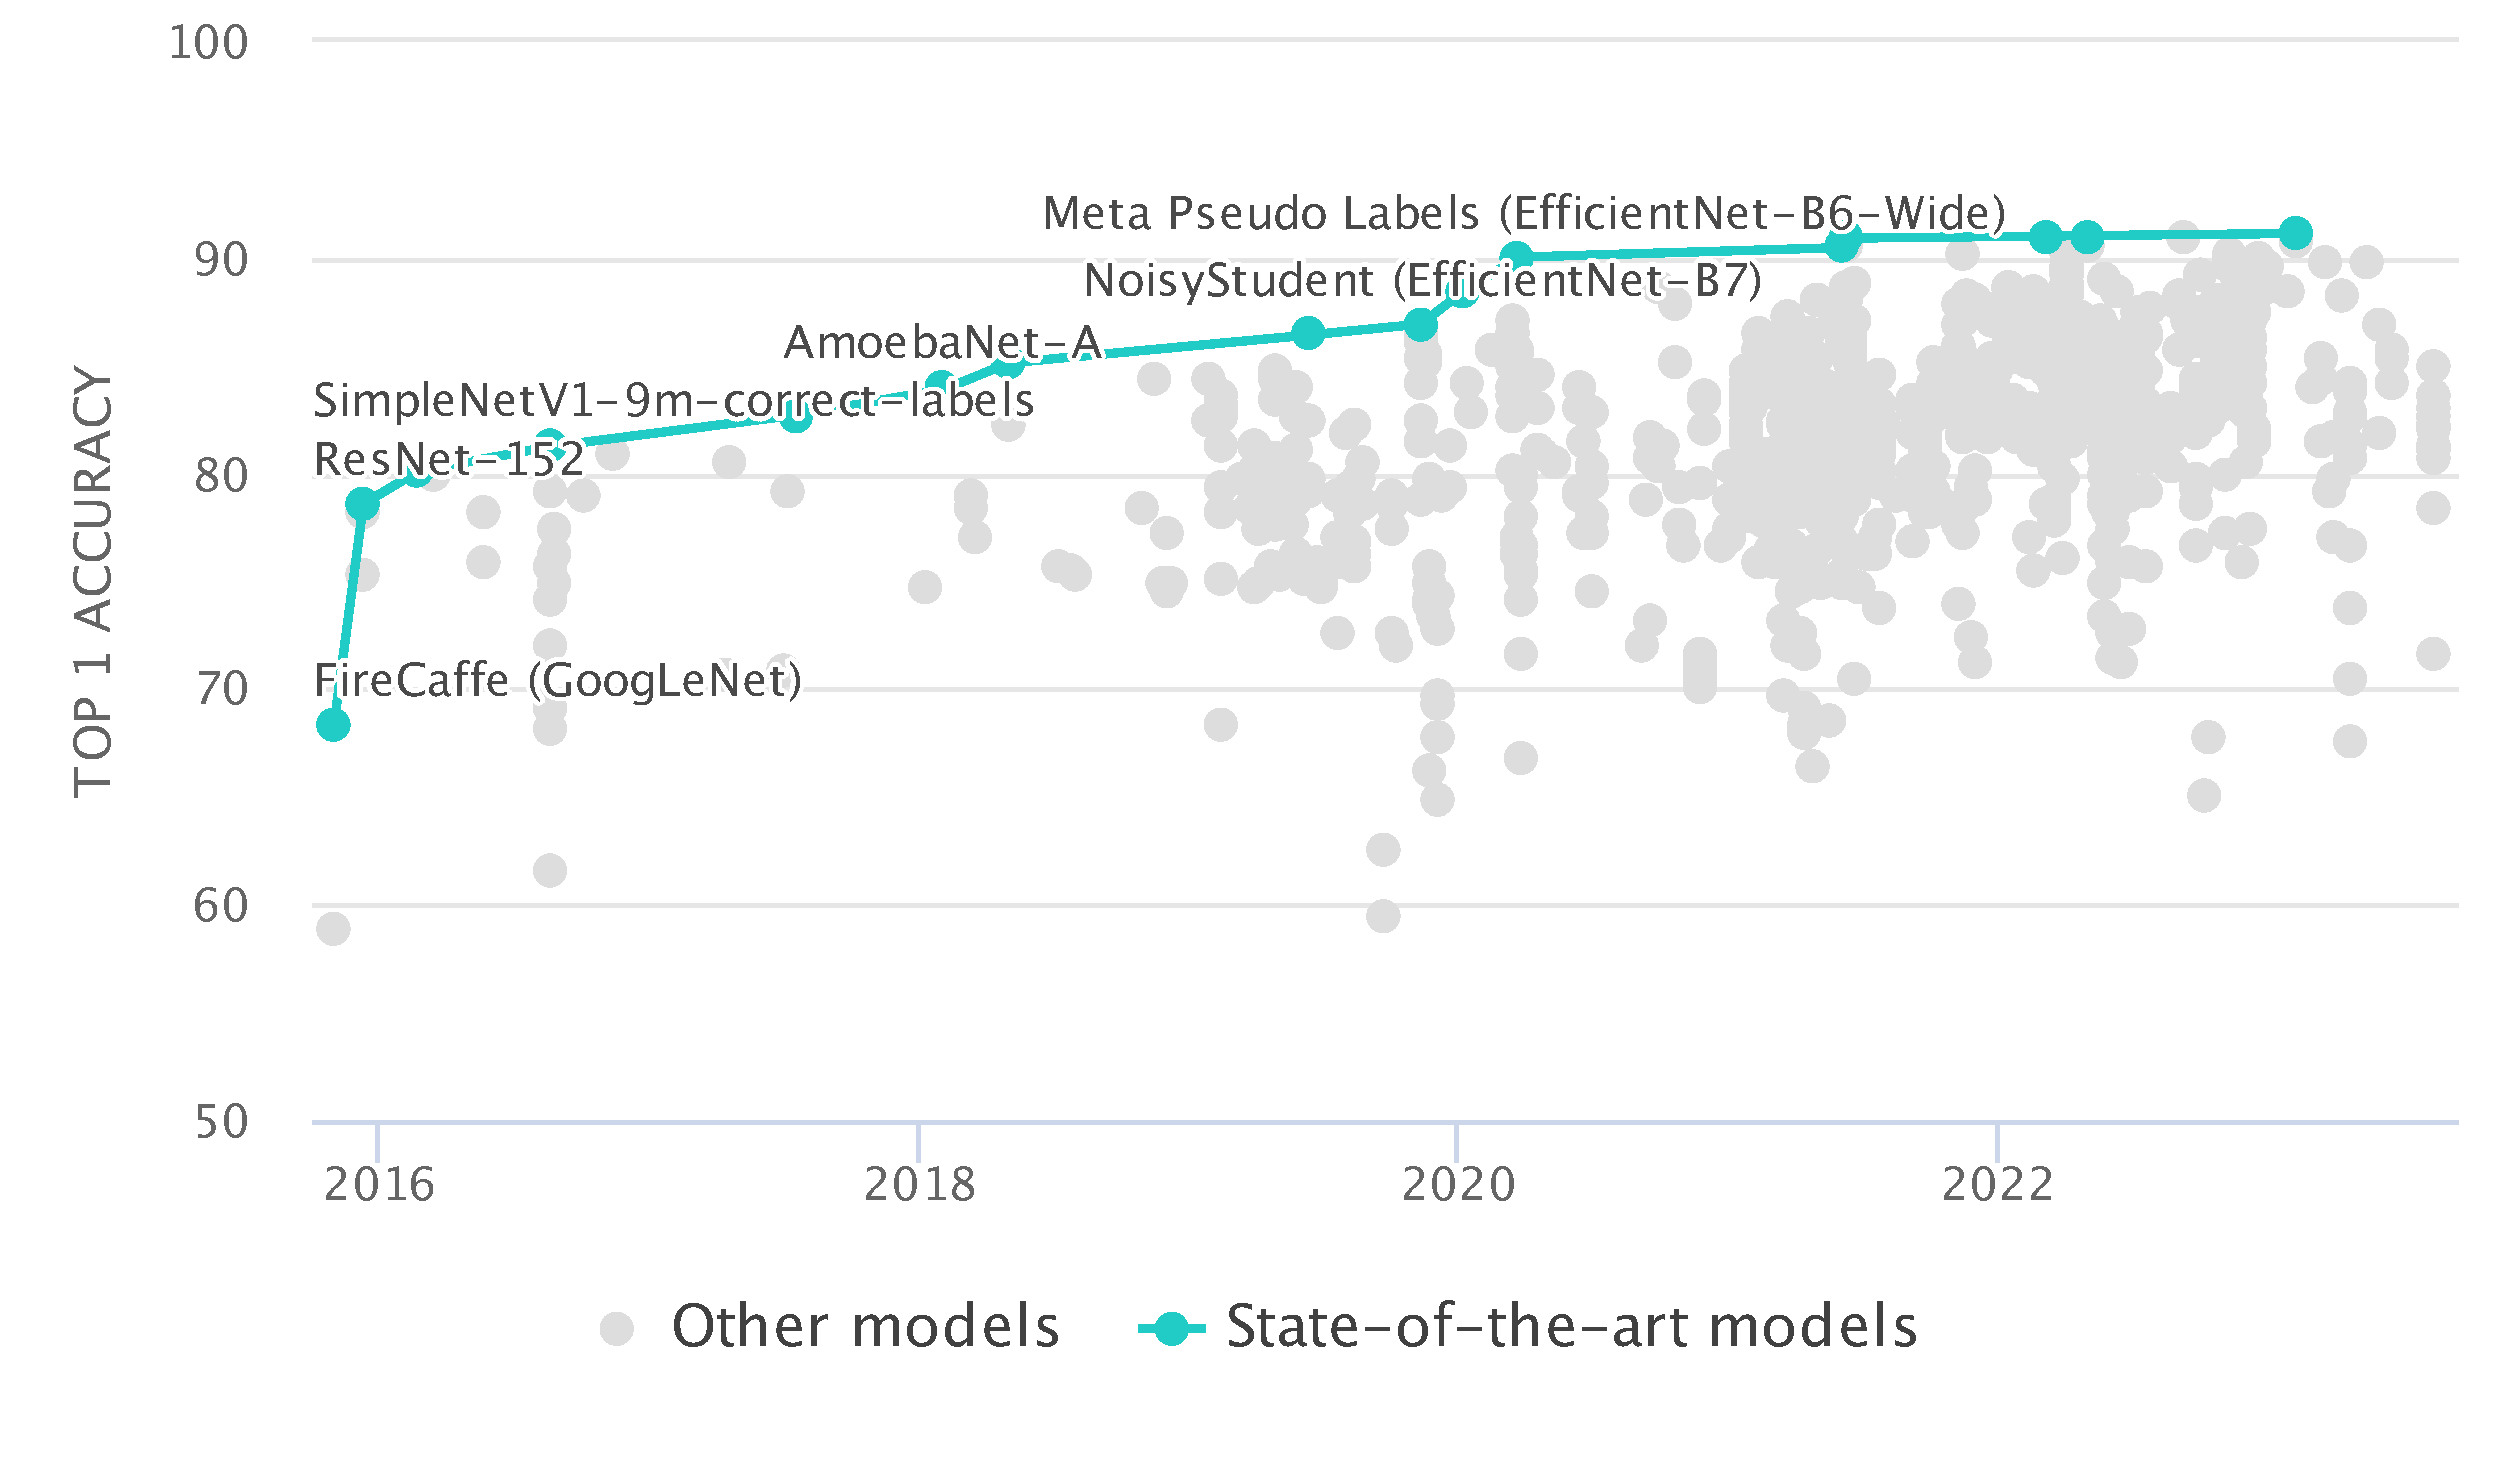
\includegraphics[width=0.8\textwidth]{examples/imagenet.pdf}
    \centering
    \caption{近年来图像分类网络的发展}
    \label{fig:imagenet}
\end{figure}

然而,深度学习的快速发展也带来了对数据崭新的需求。由于深度网络会将输入数据(如图像、文本、语音、视频等)编码为若干高维度的矢量,那么对于大量输入数据编码得到的矢量数据来说,如何有效存储它们就成为了一大难点。另一方面,人类难以理解这些矢量的含义,于是如何分析、比较这些矢量并输出结果又成为另一大难点。这些问题是传统关系型数据库无法解决的,关系型数据库只适合存储结构化数据而非多种数据格式的矢量,另外关系型数据库也不支持对矢量进行分析和计算。

基于上述原因,矢量数据库应运而生。矢量数据库以矢量的形式存储数据,其中每条矢量代表代表一个单独的样本,可能是一张图像或一句文本高维表示,并可能包含一些描述性的集合。在深度学习中,一条矢量也通常被叫做“特征”。为了实现高效的矢量存储和查找,矢量数据库实现了高效的矢量索引策略,便于通过比较矢量之间的相似度来进行相似性搜索。

目前,矢量数据库的发展还处于起步阶段,尚不存在统一的解决方案。国内一些代表性的厂商如AI领域的商汤、旷视,和互联网企业阿里巴巴、华为、京东等,这些企业各自形成了自己的矢量数据库系统。不过,当前的矢量数据库也开始出现统一规范的查询语言,并逐步与传统数据库一样实现了对数据的增删改查能力。另外,当前的矢量数据库也向着分布式、云原生的方向发展,未来的矢量数据库的扩展能力会进一步加强,单机的资源消耗和成本会进一步降低。

与传统数据库相比,矢量数据库有以下不同:

\begin{itemize}
\item 存储数据的类型和格式不同。关系数据库是为适合表的结构化数据而设计的,数据通常被组织成表格的形式,不同的属性组织成若干列,数据则以字段形式存在表格行中。矢量数据库则是为非结构化数据设计的,用于存储对象的高维信息表示。

\item 数据规模更大。传统的关系型数据库管理1亿条数据已经是拥有很大的业务流量,而在矢量数据库中通常会需求更多数据;同时,一条矢量通常就有很大的规模,例如ResNet-50的输出就有2048个维度,进一步增加了空间需求。对于海量级别的数据来说,矢量数据库需要有支持分布式扩展的能力。

\item 查询方式不同。传统的数据库基于关系模型进行查询,在关系模型中,通过关系表示实体与实体之间的联系,然后基于关系数据集合进行数据的查询、更新以及控制等操作查询。这通常是一种精确查找,即查询完全符合某种或某些条件的结果。而矢量数据库基于矢量进行查询,其依赖的是矢量之间的度量函数,如余弦相似度等。这通常是一种近似查询,即查询与条件相近的结果,这对计算能力要求非常高。
\end{itemize}